\documentclass[/home/jesse/Analysis/FemtoAnalysis/AnalysisNotes/AnalysisNoteJBuxton.tex]{subfiles}
\begin{document}

\subsection{Momentum Resolution Corrections}
\label{MomentumResolutionCorrections}

Finite track momentum resolution causes the reconstructed momentum of a particle to smear around the true value.
This, of course, also holds true for V0 particles.
The effect is propagated up to the pairs of interest, which causes the reconstructed relative momentum (\krec) to differ from the true momentum (\ktrue).
Smearing of the momentum typically will result in a suppression of the signal.  More specifically, the smearing will broaden the signal, which would cause a decrease in the extracted radius of the system.

The effect of finite momentum resolution can be investigated using the HIJING MC data, for which both the true and reconstructed momenta are available.
Figure \ref{fig:TrueVsRecLamKchP} shows sample \ktrue vs. \krec plots for \LamKpm 0-10\% analyses; Figure \ref{fig:TrueVsRecLamKchP:a} was generated using same-event pairs, while Figure \ref{fig:TrueVsRecLamKchP:b} was generated using mixed-event pairs (with N$_{mix}$ = 5).  


\begin{figure}[h!]
  \centering
  %%----start of first subfigure---  
  \subfloat[Same Event Pairs (\LamKpm, 0-10\% Centrality)]{
    \label{fig:TrueVsRecLamKchP:a}
    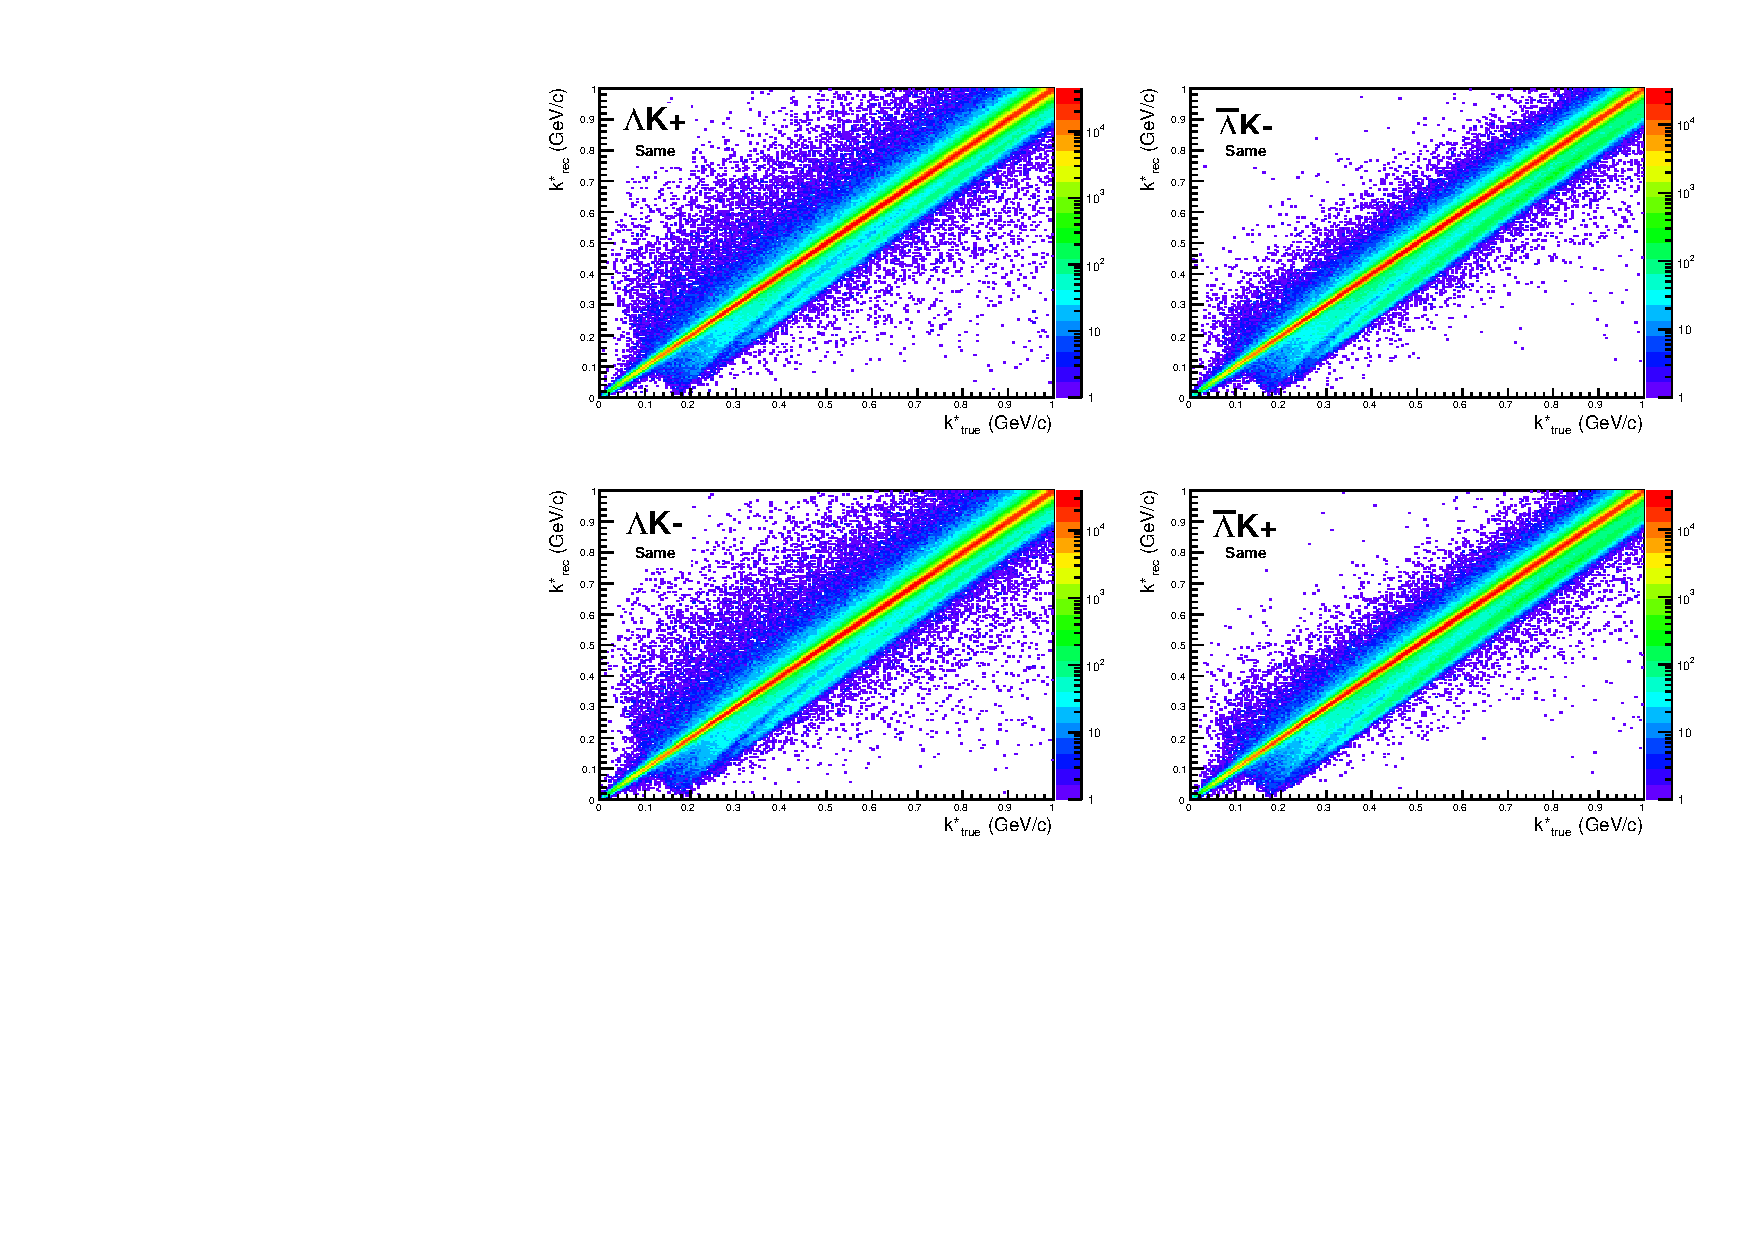
\includegraphics[width=0.7\textwidth]{5_Fitting/Figures/canKStarTrueVsRecLamKchP_0010Same.pdf}}\\
  %%----start of second subfigure---
  \subfloat[Mixed Event Pairs (\LamKpm, 0-10\% Centrality)]{
    \label{fig:TrueVsRecLamKchP:b}
    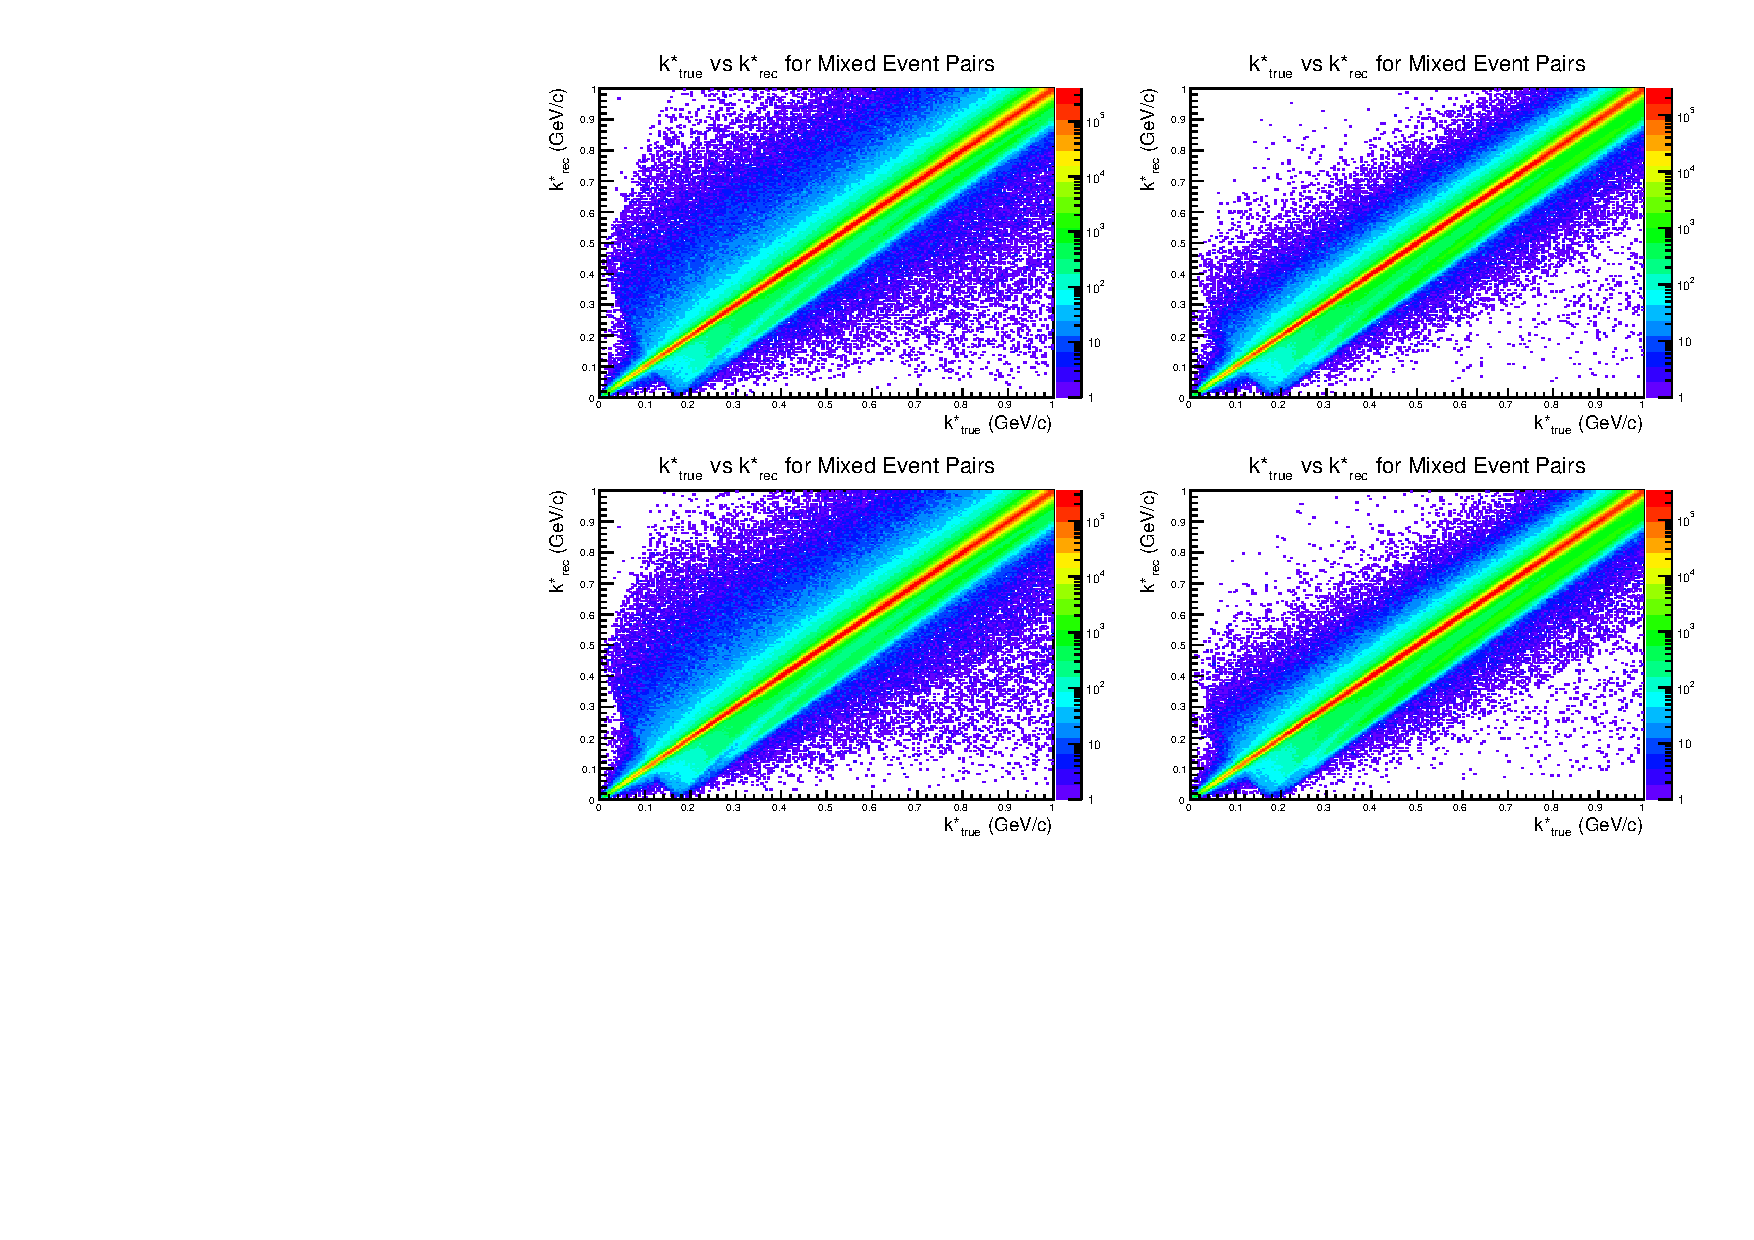
\includegraphics[width=0.7\textwidth]{5_Fitting/Figures/canKStarTrueVsRecLamKchP_0010Mixed.pdf}}
  %%----overall caption----
  \caption[Momentum Resolution: Sample \ktrue vs. \krec]{Sample \ktrue vs. \krec plots from MC HIJING events for \LamKpm 0-10\% analyses.  The structure which appears around \krec = \ktrue - 0.15 GeV/$c$ is mainly caused by \Ks contamination in our \LamALam sample.  The remaining structure not distributed about \krec = \ktrue is due to $\pi$ and $e$ contamination in our \Kpm sample.  These contaminations are more clearly visible in Figure \ref{fig:TrueVsRecLamKchP_MisID}}
  \label{fig:TrueVsRecLamKchP}
\end{figure}


If there are no contaminations in our particle collection, the plots in Figure \ref{fig:TrueVsRecLamKchP} should be smeared around \ktrue = \krec; this is mostly true in our analyses.
However, there are some interesting features of our results which demonstrate a small (notice the log-scale on the z-axis) contamination in our particle collection.
The structure around \krec = \ktrue - 0.15 GeV/$c$ is mainly caused by \Ks contamination in our \LamALam sample.
The remaining structure not distributed about \krec = \ktrue is due to $\pi$ and $e$ contamination in our K$^{\pm}$ sample.
These contaminations are more visible in Figure \ref{fig:TrueVsRecLamKchP_MisID}, which show \krec vs. \ktrue plots (for a small sample of the \LamKchP 0-10\% central analysis), for which the MC truth (i.e. true, known identity of the particle) was used to eliminate misidentified particles in the K$^{+}$(a) and $\Lambda$(b) collections. (NOTE: This is an old figure and is for a small sample of the data.  A new version will be generated shortly.  It, nonetheless, demonstrates the point well).


\begin{figure}[h!]
  \centering
  %%----start of first subfigure---  
  \subfloat[(Top Left) All misidentified \KchP excluded.  (Bottom Left) All misidentified \Lam and \KchP excluded.  (Right) The difference of (Top Left) - (Bottom Left), which reveals the contamination in our \Lam collection. The structure which appears around \krec = \ktrue - 0.15 GeV/$c$ is mainly caused by \Ks contamination in our \LamALam sample.]{
    \label{fig:TrueVsRecLamKchP_MisID:a}
    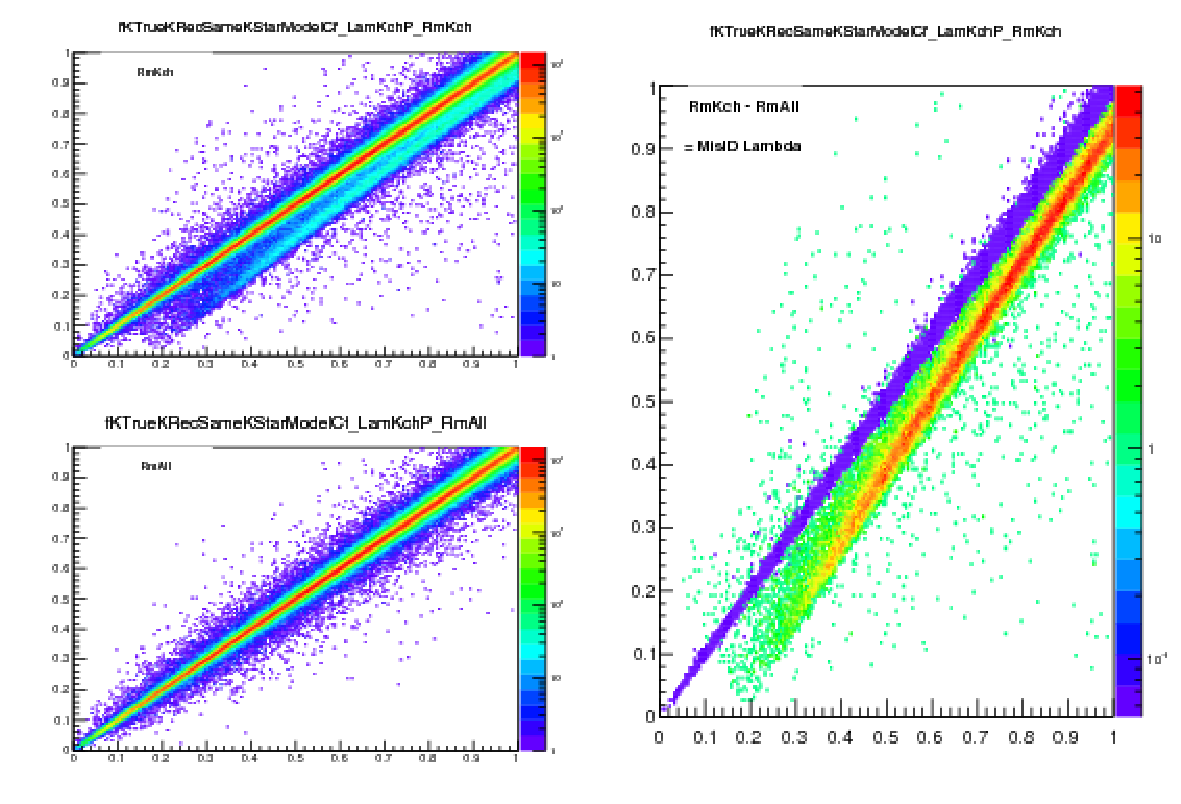
\includegraphics[width=0.7\textwidth]{5_Fitting/Figures/RmKchVsRmAll.pdf}}\\
  %%----start of second subfigure---
  \subfloat[(Top Left) All misidentified \Lam excluded.  (Bottom Left) All misidentified \Lam and \KchP excluded. (Right) The difference of (Top Left) - (Bottom Left), which reveals the contamination in our \KchP collection. The structure not distributed about \krec = \ktrue is due to $\pi$ and $e$ contamination in our \KchP sample.]{
    \label{fig:TrueVsRecLamKchP_MisID:b}
    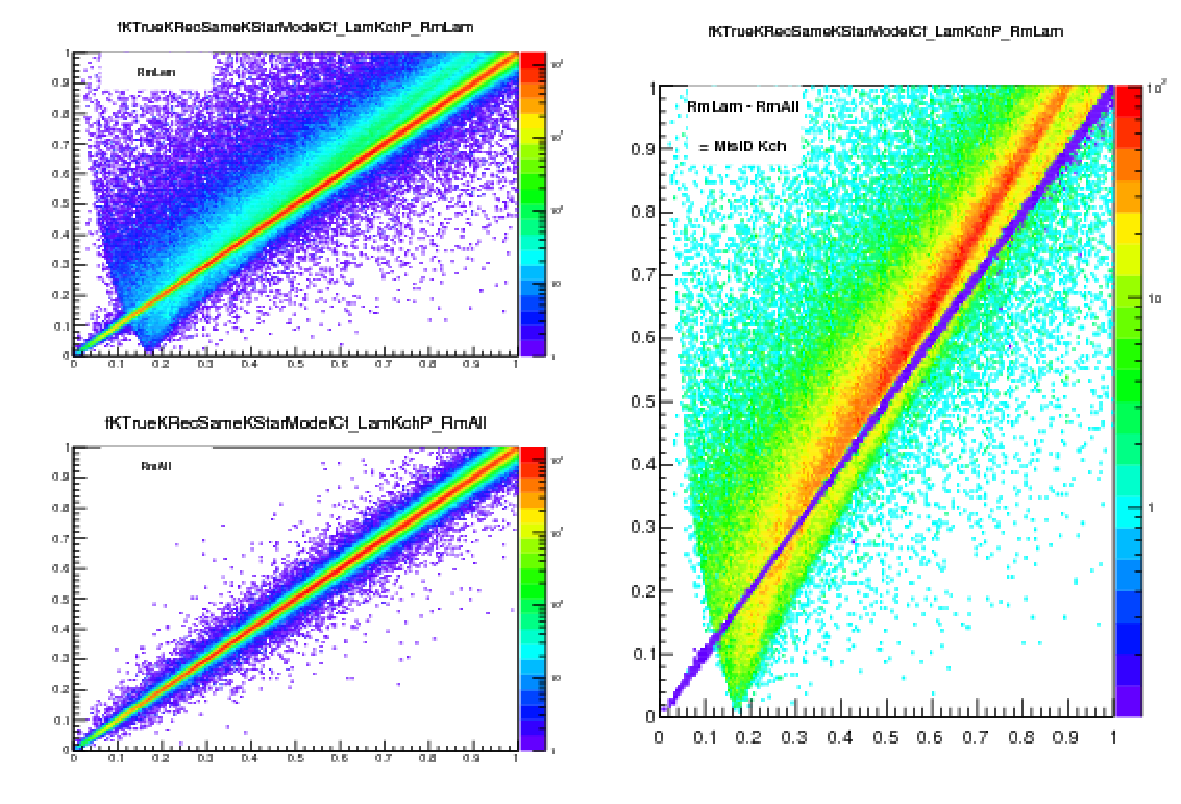
\includegraphics[width=0.7\textwidth]{5_Fitting/Figures/RmLamVsRmAll.pdf}}
  %%----overall caption----
  \caption[Particle Contaminations Visible in \ktrue vs. \krec]{In the figure, the y-axis = \krec, and the x-axis = \ktrue.
(Left) \krec vs. \ktrue plots for a small sample of the \LamKchP 0-10\% central analysis, MC truth was used to eliminate misidentified particles in the \KchP(a) and \Lam(b) collections. 
(Right) The difference of the top left and bottom left plots.
Contaminations in our particle collections are clearly visible. Figure (a) demonstrates a \Ks contamination in our \Lam collection; Figure (b) demonstrates a $\pi$ and $e^{-}$ contamination in our \Kpm collection.}
  \label{fig:TrueVsRecLamKchP_MisID}
\end{figure}


Information gained from looking at \krec vs ktrue can be used to apply corrections to account for the effects of finite momentum resolution on the correlation functions.
A typical method (``Ratio'' method) involves using the MC HIJING data to build two correlation functions, $C_{\mathrm{Rec}}(k^{*})$ and $C_{\mathrm{True}}(k^{*})$, using the generator-level momentum (\ktrue) and the measured detector-level momentum (\krec).
The data is then corrected by multiplying by the ratio, $C_{\mathrm{True}}/C_{\mathrm{Rec}}$, before fitting.
This essentially unsmears the data, which then can be compared directly to theoretical predictions and fits.
Although this is conceptually simple, there are a couple of big disadvantages to this method.
First, HIJING does not incorporate final-state interactions, so weights must be used when building same-event (numerator) distributions.
These weights account for the interactions, and, in the absence of Coulomb interactions, can be calculated using Eq. \ref{eqn:LednickyEqn}.
Of course, these weights are valid only for a particular set of fit parameters.
Therefore, in the fitting process, during which the fitter explores a large parameter set, the corrections will not remain valid.
As such, applying the momentum resolution correction and fitting becomes a long and drawn out iterative process.
An initial parameter set is obtained (through fitting without momentum resolution corrections, theoretical models, or a good guess), then the MC data is analyzed to obtain correlation functions needed to calculate the correction factor, the data is fit using the correction factor, a refined parameter set is extracted, the MC data is analyzed again to obtain the new correction factor, etc.
This process continues until the parameter set stabilizes.
The second issue concerns statistics.
With the MC data available on the grid, we were not able to generate the statistics necessary to use the raw $C_{\mathrm{True}}/C_{\mathrm{Rec}}$ ratio.
The ratio was not stable, and when applied to the data, obscured the signal.
Attempting to fit the ratio to use to generate the corrections also proved problematic.
However, as HIJING does not include final-state interactions, the same-event and mixed-event pairs are very similar (with the exception of things like energy and momentum conservation, etc).
Therefore, one may build the numerator distribution using mixed-event pairs.
This corresponds, more or less, to simply running the weight generator through the detector framework.

A second approach (``Matrix'' method) is to use information gained from plots like those in Figure \ref{fig:TrueVsRecLamKchP}, which can be considered response matrices.
The response matrix describes quantitatively how each \krec bin receives contributions from multiple \ktrue bins, and can be used to account for the effects of finite momentum resolution.
With this approach, the resolution correction is applied on-the-fly during the fitting process by propagating the theoretical correlation function (fit) through the response matrix, according to:  

\begin{equation}
  C_{\mathrm{Fit}}(k^{*}_{\mathrm{Rec}}) = \dfrac{\sum\limits_{k^{*}_{\mathrm{True}}}M_{k^{*}_{\mathrm{Rec}},k^{*}_{\mathrm{True}}}C_{\mathrm{Fit}}(k^{*}_{\mathrm{True}})}{\sum\limits_{k^{*}_{\mathrm{True}}}M_{k^{*}_{\mathrm{Rec}},k^{*}_{\mathrm{True}}}}
\label{eqn:MomResCorrection}
\end{equation}

where $M_{k^{*}_{\mathrm{Rec}},k^{*}_{\mathrm{True}}}$ is the response matrix (Figure \ref{fig:TrueVsRecLamKchP}), $C_{\mathrm{Fit}}(k^{*}_{\mathrm{True}})$ is the fit binned in \ktrue, and the denominator normalizes the result.

Equation \ref{eqn:MomResCorrection} describes that, for a given \krec bin, the observed value of $C(k^{*}_{\mathrm{Rec}})$ is a weighted average of all $C(k^{*}_{\mathrm{True}})$ values, where the weights are the normalized number of counts in the [\krec, \ktrue] bin.
As seen in Figure \ref{fig:TrueVsRecLamKchP}, overwhelmingly the main contributions comes from the \krec = \ktrue bins.
Although the correction is small, it is non-negligible for the low-\kstar region of the correlation function.

Here, the momentum resolution correction is applied to the fit, not the data.
In other words, during fitting, the theoretical correlation function is smeared just as real data would be, instead of unsmearing the data.
This may not be ideal for the theorist attempting to compare a model to experimental data, but it leaves the experimental data unadulterated.
The current analyses use this second approach to applying momentum resolution corrections because of two major advantages.  First, the MC data must be analyzed only once, and no assumptions about the fit are needed.  Secondly, the momentum resolution correction is applied on-the-fly by the fitter, delegating the iterative process to a computer instead of the user.

The two methods described above, Ratio and Matrix, should reproduce the same results at the parameter set used to generate the $C_{\mathrm{True}}/C_{\mathrm{Rec}}$ needed for the Ratio method.  Figure \ref{fig:MomResMethodComp} shows that the two methods converge as the binning size is decreased.


\begin{figure}[h!]
  \centering
  %%----start of first subfigure---  
  \subfloat[\LamKchP]{
    \label{fig:MomResMethodComp:a}
    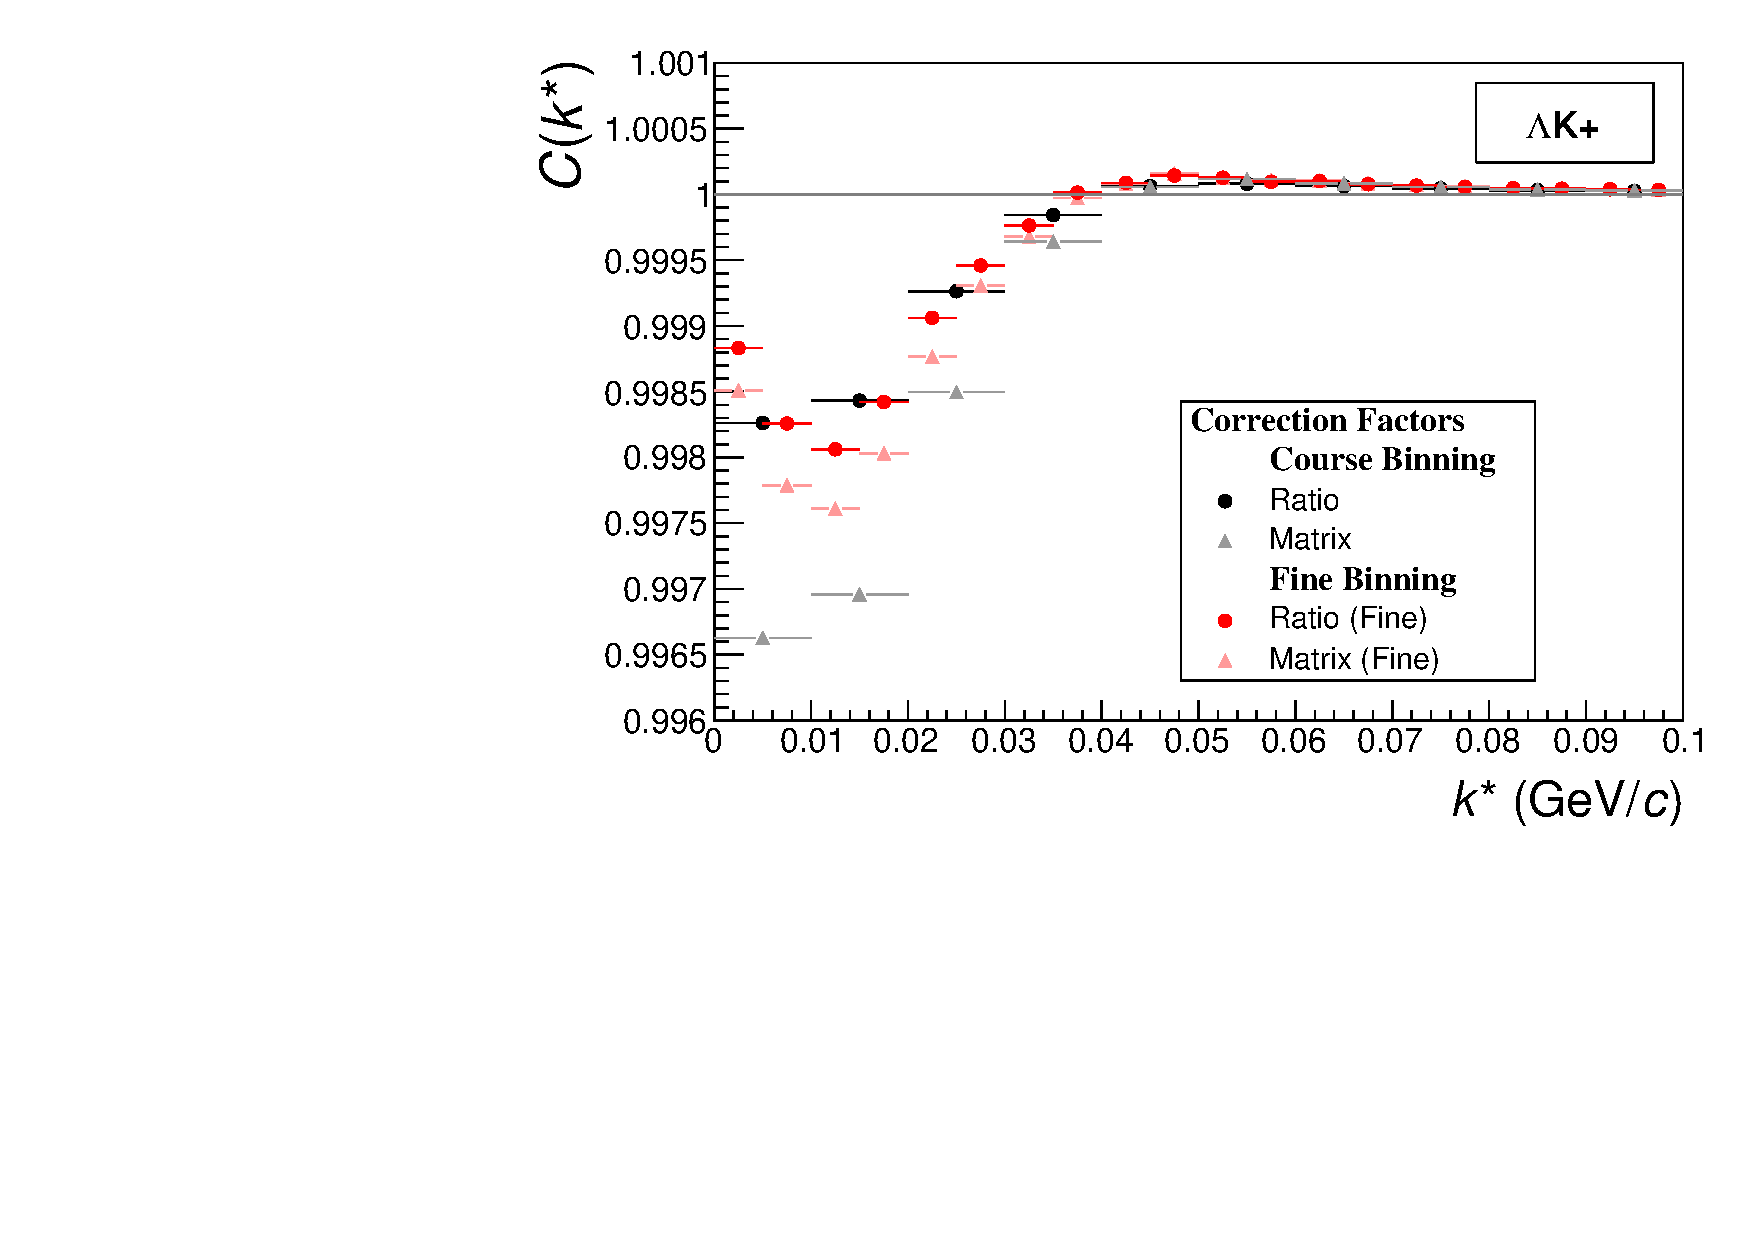
\includegraphics[width=0.49\textwidth]{/home/jesse/Analysis/FemtoAnalysis/AnalysisNotes/5_Fitting/Figures/CorrectionFactors_CompareFine_LamKchP.pdf}}
  %%----start of second subfigure---
  \subfloat[\ALamKchM]{
    \label{fig:MomResMethodComp:b}
    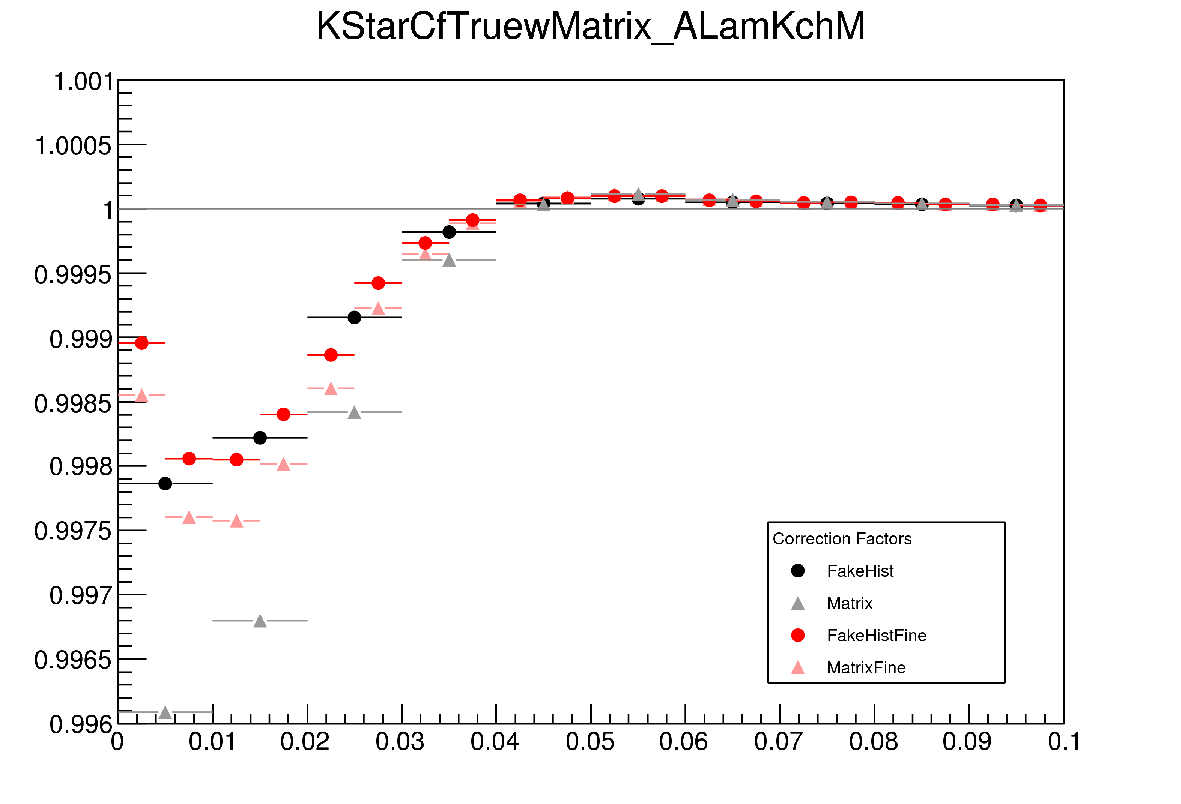
\includegraphics[width=0.49\textwidth]{/home/jesse/Analysis/FemtoAnalysis/AnalysisNotes/5_Fitting/Figures/CorrectionFactors_CompareFine_ALamKchM.pdf}}  
  \\  
  %%----start of third subfigure---
  \subfloat[\LamKchM]{
    \label{fig:MomResMethodComp:c}
    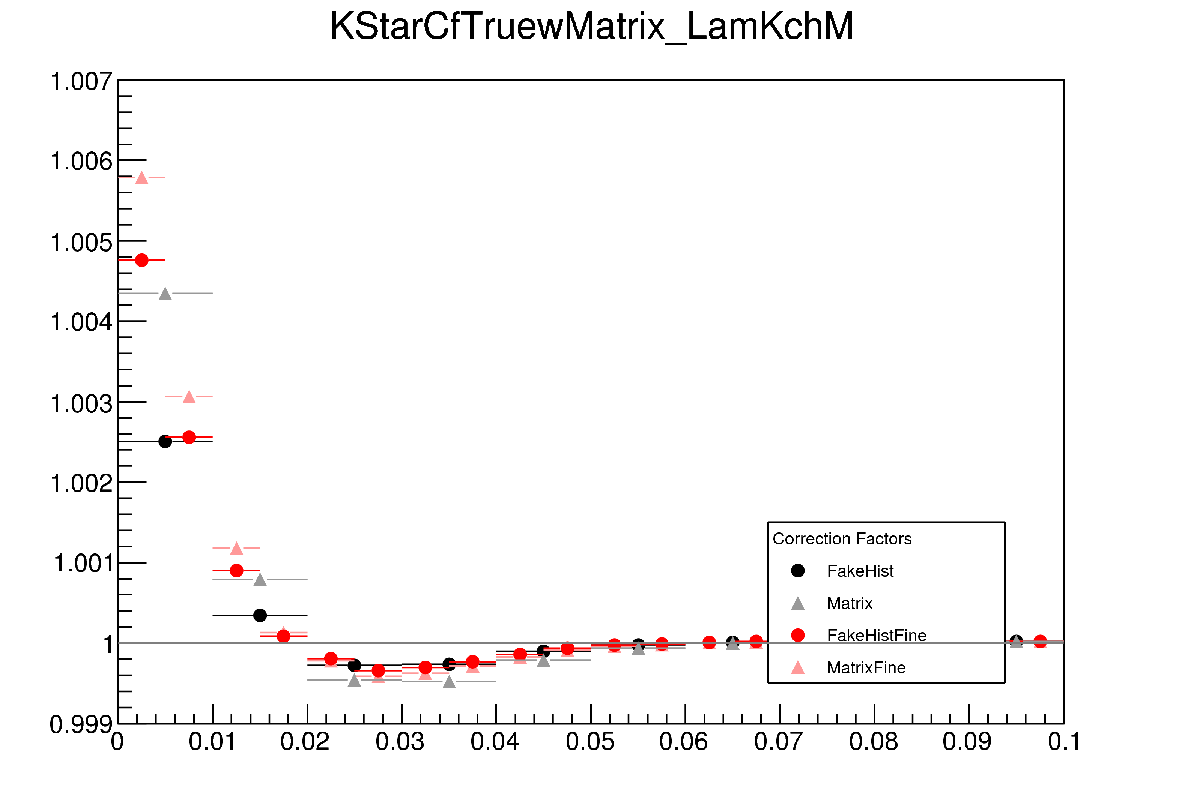
\includegraphics[width=0.49\textwidth]{/home/jesse/Analysis/FemtoAnalysis/AnalysisNotes/5_Fitting/Figures/CorrectionFactors_CompareFine_LamKchM.pdf}}  
  %%----start of fourth subfigure---
  \subfloat[\ALamKchP]{
    \label{fig:MomResMethodComp:d}
    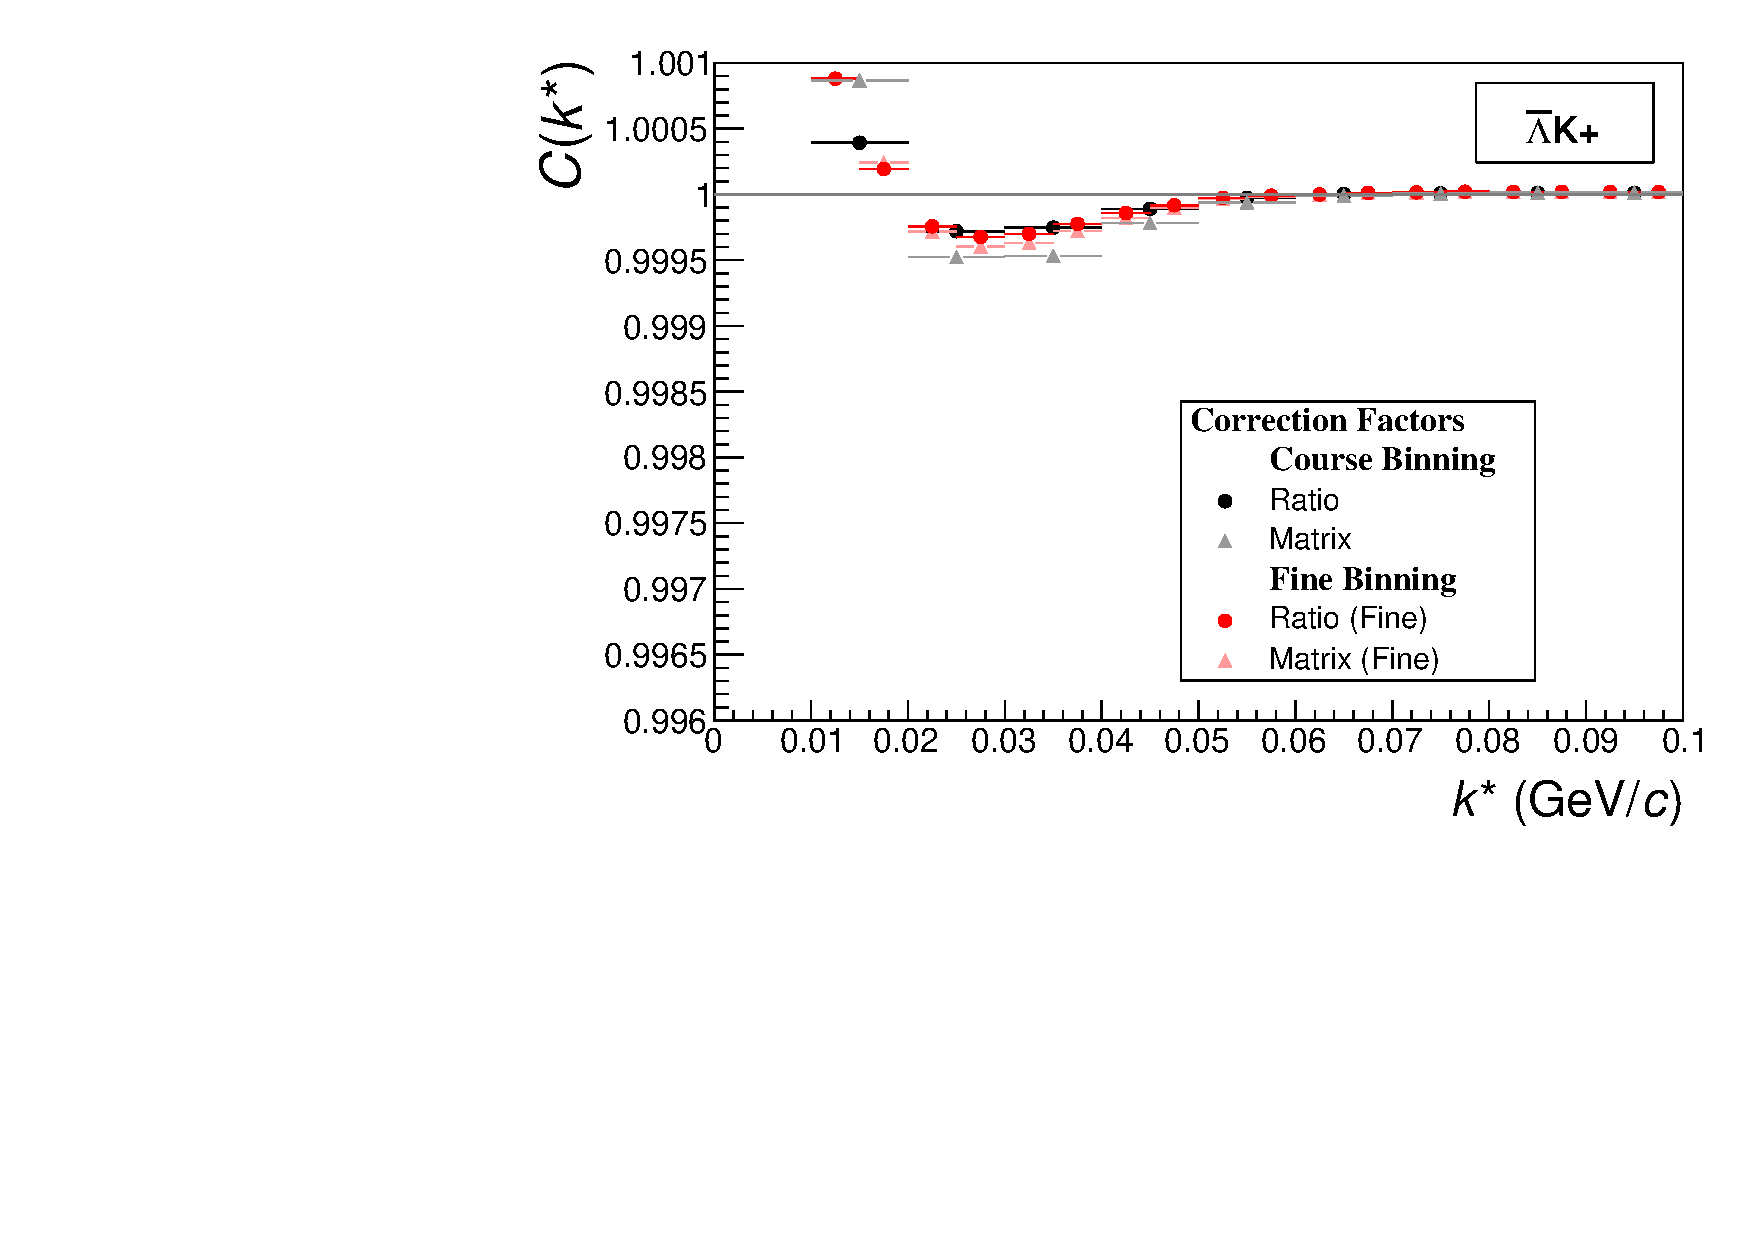
\includegraphics[width=0.49\textwidth]{/home/jesse/Analysis/FemtoAnalysis/AnalysisNotes/5_Fitting/Figures/CorrectionFactors_CompareFine_ALamKchP.pdf}}          
  %%----overall caption----
  \caption[Momentum Resolution Corrections: Methods Comparison]{Comparison of the two methods, Ratio and Matrix, for accounting for momentum resolution effects with HIJING.  The Ratio method corresponds to the ``FakeHist'' histograms (circles), while the Matrix method corresponds to the ``Matrix'' histograms (triangles).  Black shows a course binning, while red shows a finer binning.}
  \label{fig:MomResMethodComp}
\end{figure}




\clearpage



\end{document}